\chapter{Analisi spettrometrica}
\label{ch:spettro}

La determinazione delle specie reattive prodotte dal plasma a pressione atmosferica può essere effettuata tramite misure spettrometriche della sorgente in funzione su un bersaglio.
Gli effetti del trattamento al plasma si pensano dovuti alla presenza di ROS e RNS, quindi vengono raccolte misure nel range di lunghezze d'onda utili ad osservare le emissioni di molecole di \ce{OH} (\SI{305.00}-\SI{313.00}{\nano\meter}), \ce{N_{2}} (\SI{280.00}-\SI{500.00}{\nano\meter}) e \ce{NO} (\SI{220.0}-\SI{290.0}{\nano\meter}) (vedi articoli).

I prototipi di sorgente sviluppati permettono di variare il range dei parametri di funzionamento, in modo da modulare l'intensità del trattamento. Per verificare come cambia lo spettro in base alle diverse modalità di funzionamento, si osservano la variazione nell'intensità delle emissioni al cambiare di frequenza e tempo di apertura del circuito.

Si vuole osservare l'intensità relativa delle righe al variare del gas in ingresso, quindi la sorgente viene azionata con diverse miscele di gas. La misura standard viene effettuata con flusso di \ce{He}, nella solita modalità di funzionamento della sorgente. Vengono poi predisposte due ulteriori modalità di misura dove il gas viene fatto gorgogliare in una soluzione di acqua o di ammoniaca prima dell'inserimento all'uscita della sorgente, per arricchire i prodotti delle reazioni di ioni contenenti, rispettivamente, ossigeno o azoto.

A partire dalla forma delle righe di alcune specie molecolari, è inoltre possibile stimare la temperatura rotazionale alla quale avviene l'emissione misurata. Le emissioni dovute alla molecola \ce{OH} o \ce{N_2} sono varie righe dalle intensità variabili a seconda della temperatura delle molecole, misurando l'intensità relativa dei picchi si può ricavare la temperatura rotazionale delle molecole.

\section{Setup di acquisizione}
La misura viene effettuata tramite uno spettrometro IsoPlane dalla lunghezza focale di \SI{320}{\milli\meter}, con tre diversi reticoli: \SI{150}, \SI{1200} e \SI{2400}{g/\milli\meter}, corrispondenti alle risoluzioni di ... .
La risoluzione maggiore viene utilizzata per acquisire le righe \ce{OH} e \ce{N_{2,\text{rot}}}, mentre per acquisire lo spettro totale vengono utilizzati i reticoli a piccola e media risoluzione.

Lo spettrometro è accoppiato ad una telecamera PIXIS di $2048 \times $ ... pixels quadrati dal lato di ... \si{\micro\meter}, con un massimo di \SI{65000} conteggi per il singolo canale.
La luce viene raccolta da una lente in quarzo di focale ... e diametro ... , portata da una fibra ottica dallo spessore di ... e lunghezza di ... e collegata all'entrata dello spettrometro.

Per l'acquisizione viene posizionata la sorgente in funzione a distanza di \SI{1}{\centi\metre} dal bersaglio in metallo (collegato a terra) con l'ottica focalizzata sul flusso di gas, come in foto \ref{fig:app}. Vengono distinte due posizioni dell'ottica:
\begin{itemize}
 \item posizione 1 = obiettivo sull'uscita della sorgente
 \item posizione 2 = obiettivo sul punto di impatto del plasma sulla sorgente, ad \SI{1}{\centi\meter} dall'uscita della sorgente
\end{itemize}
.

\begin{figure}
\centering
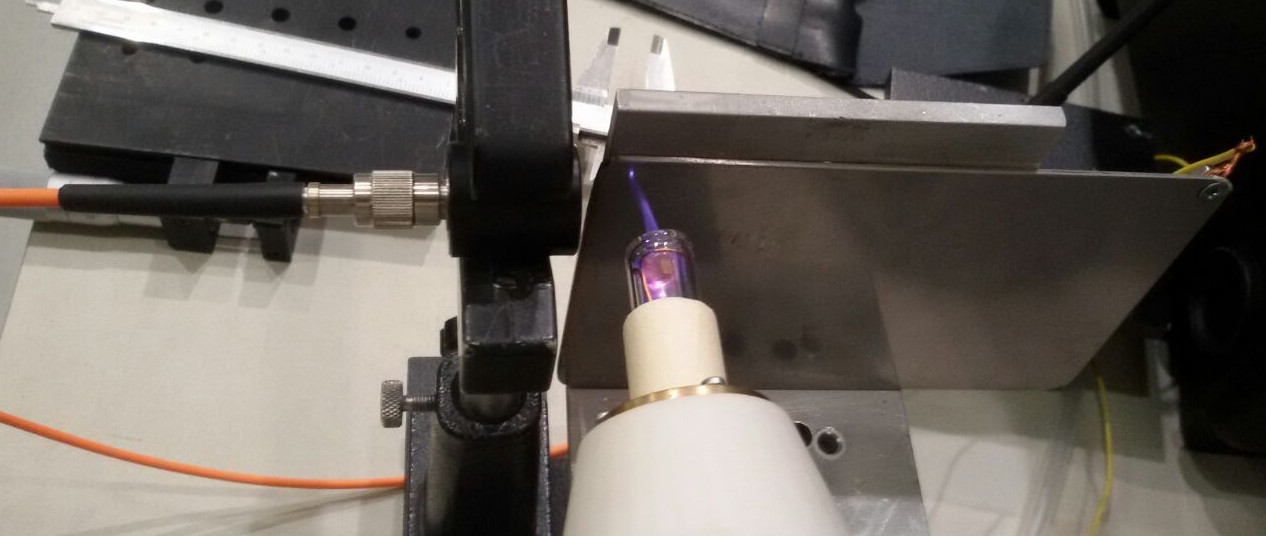
\includegraphics[width=.6\textwidth]{Immagini/apparato.jpg}
\caption{Configurazione per le misure spettrometriche. Si vedono la sorgente in funzione, il bersaglio in metallo, obiettivo e fibra ottica a sinistra.}
\label{fig:app}
\end{figure}

Per ogni misura viene stabilito un tempo di acquisizione idoneo ad avere un numero ottimale di eventi, evitando la saturazione dei singoli canali. Una volta stabilito il tempo viene eseguita una misura di fondo, a sorgente spenta, e successivamente viene avviata la misura con sorgente attiva.

Per la sorgente vengono utilizzati sia il prototipo precedente, \textbf{prototipo 1} , sia il prototipo svilupato durante questo lavoro, \textbf{prototipo 2}.

Vengono inoltre provate tre diverse modalità di funzionamento della sorgente, variando frequenza e tempo di chiusura del circuito, mostrate in Tabella \ref{tab:setsorgente}.
Il flusso del gas di elio viene mantenuto pari a \SI{2}{\liter/\minute}.

\begin{table}
 \centering
 \begin{tabular}{cc}
 \toprule
 $f$ [\si{\kilo\hertz}]  &$\Delta t$ [\si{\micro\second}]\\
 \midrule
 5  &15\\
 10 &10\\
 15 &10\\
 \bottomrule
 \end{tabular}
 \caption{Parametri di funzionamento utilizzati per le diverse misure.}
 \label{tab:setsorgente}
\end{table}



\section{Presentazione ed analisi misure}
Per entrambe le sorgenti, l'analisi prevede il riconoscimento delle emissioni misurate, il confronto delle intensità variando distanza e parametri di funzionamento della sorgente, il confronto delle intensità variando il gas immesso, la stima delle temperature rotazionali delle molecole \ce{OH} e \ce{N_2}.

\subsection{Riconoscimento righe}
L'output dello spettrometro viene letto tramite routine IDL ed il riconoscimento dei picchi viene effettuato tramite la classe TSpectrum presente nelle librerie ROOT. Ogni misura viene confrontata con uno spettro di background preso con lo stesso tempo di acquisizione e sorgente spenta, riuscendo così ad escludere i picchi dovuti al fondo.
In figura \ref{fig:spettrotot} si vedono le principali righe estrapolate dalle acquisizioni, in particolare si vedono le righe relative ad \ce{NO}, \ce{OH}, \ce{H_{2}} e \ce{N_{2}}, tabulate in Tabella \ref{tab:spettrotot} .

\begin{figure}
\centering
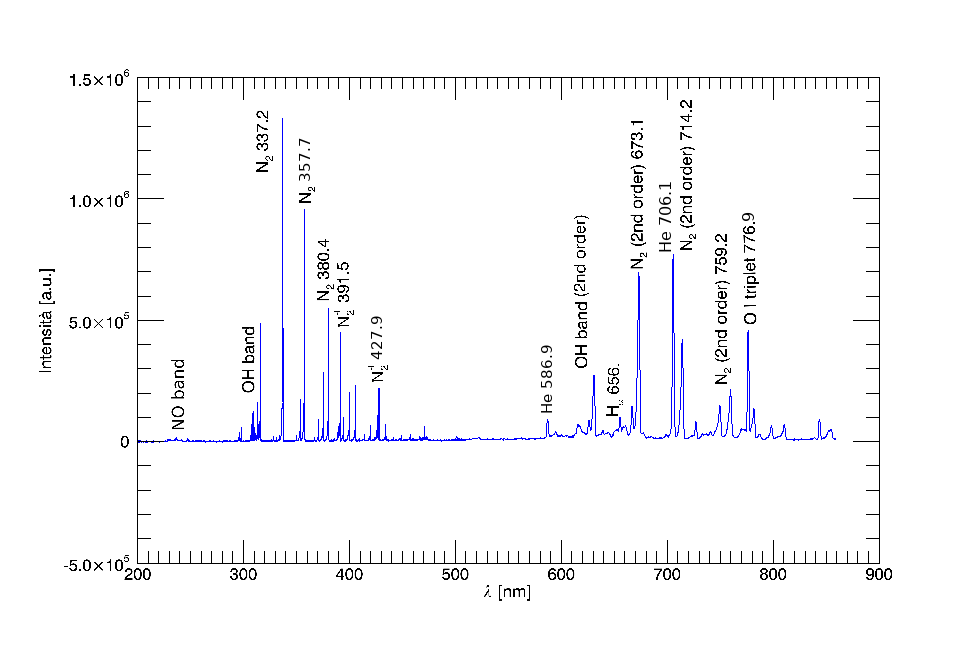
\includegraphics[width=0.99\textwidth]{Immagini/spettrotot_unico_label_def.png}
\caption{Spettro acquisito con condizioni di misura standard ($f = \SI{5}{\kilo\hertz}$ e $\Delta t = \SI{16}{\micro\second}$), obiettivo puntato vicino l'uscita del gas dalla sorgente.}
\label{fig:app}
\end{figure}

\begin{table}
\centering
 \begin{tabular}{ccc}
  \toprule
                            &$\lambda$ \text{[}\si{\nano\meter}\text{]} &\text{I [arb.u.]}\\
  \midrule
  \multirow{2}*{\ce{OH}}    &308.3  &106\\
                            &309.1  &113\\
  \midrule
  \multirow{5}*{\ce{N_2}}   &315.9  &381\\
                            &337.2  &1000\\
                            &357.7  &722\\
                            &375.6  &232\\
                            &380.4  &423\\
  \midrule
  \multirow{2}*{\ce{N_2^+}} &391.5  &355\\
                            &427.9  &180\\
  \midrule
  \multirow{4}*{\ce{NO}}    &236.3  &27\\
                            &237.0  &26\\
                            &247.0  &28\\
                            &247.8  &27\\
  \midrule
  \ce{H_{\alpha}}           &656.0  &113\\
  \midrule
  \multirow{2}*{\ce{He}}    &586.9  &122\\
                            &706.1  &649\\
  \midrule
  \ce{O}                    &776.9  &393\\
  \bottomrule
 \end{tabular}
 \caption{Picchi rilevanti nello spettro di emissione del prototipo 1, condizioni di misura standard, posizione 1.}
 \label{tab:spettrotot}
\end{table}

L'acquisizione migliore, nella quale vengono riconosciuti più picchi, è quella mostrata in Figura \ref{fig:spettrotot}, corrispondente alla posizione 1 e condizioni standard di misura, $f = \SI{5}{\kilo\hertz}$.

\paragraph{}
Per verificare gli effetti di una diversa frequenza  nel funzionamento della sorgente vengono confrontate le intensità relative alle righe di \ce{OH} e \ce{N_2}, sommando i conteggi per le varie porzioni di spettro. Non vengono prese in considerazione le righe del gruppo relativo all'\ce{NO} in quanto troppo deboli. In Tabella \ref{tab:irel_1} i risultati, dove vengono confrontate i conteggi alle varie frequenze rispetto i conteggi ottenuti nelle condizioni standard di lavoro, $f = \SI{5}{\kilo\hertz}$. Si nota un calo evidente nei conteggi, crescente con l'aumentare della frequenza di lavoro.

Allo stesso modo viene variata la posizione dell'obbiettivo, dalla posizione 1, puntato all'uscita della sorgente, alla posizione 2, puntato all'uscita del bersaglio. I risultati sempre in Tabella \ref{tab:irel_1}, dove vengono presentati i conteggi nella posizione 2 rispetto i conteggi nella posizione 1. Viene trovato un effetto diverso sulle diverse specie, le emissioni di \ce{OH} diminuiscono molto, mentre quelle relative l'\ce{N_2} diminuiscono in maniera inferiore.

\begin{table}
 \centering
 \begin{tabular}{lcc}
 \toprule
                            &\ce{OH}  &\ce{N_2}\\
 \midrule
 f = \SI{5}{\kilo\hertz}    &1.00     &1.00\\
 f = \SI{10}{\kilo\hertz}    &0.95    &0.81\\
 f = \SI{15}{\kilo\hertz}    &0.62    &0.63\\
 \midrule
 posizione 1                &1.00        &1.00\\
 posizione 2                &0.10     &0.82\\
 \bottomrule
 \end{tabular}
 \caption{Intensità relative delle porzioni interessanti di spettro, al variare di frequenza e posizione, per il prototipo 1.}
 \label{tab:irel_1}
\end{table}


\subsection{\ce{He} + \ce{H_2O} e \ce{He} + \ce{NH_3}}
Vengono misurati gli spettri di emissione in condizioni di lavoro standard, $f = \SI{5}{\kilo\hertz}$, posizione 1, trattando il flusso di elio prima di inserirlo nella sorgente.
Per il prototipo 1, l'arricchimento di specie reattive dell'ossigeno o dell'azoto avviene facendo gorgogliare l'elio in una soluzione di acqua o ammoniaca, mantenendo un flusso in uscita dalla bombola sempre di \SI{2}{\liter/\minute}.
Le misure così acquisite presentano un'intensità molto minore per tutte le righe dello spettro e non vi sono variazioni rilevanti per le lunghezze d'onda interessate, cioè le emissioni relative ad \ce{OH} per la soluzione di acqua e relative ad \ce{N_2} per la soluzione di ammoniaca.

\subsection{Stima temperatura}
Lo spettro di emissione della molecola \ce{OH} è della forma presentata in Equazione \ref{eq:fitOH} (vedi articolo):
\begin{equation}
\centering
\begin{split}
&I_i (T) = I_{0,i} \exp{-\frac{E_n (T-T_0)}{T_0 T}} \\
&S_i(\lambda,T) = \frac{I_i(T)}{\sigma \sqrt{2\pi}} \exp{\frac{(\lambda - \lambda_i)^2}{2\sigma^2}}\\
&S(\lambda,T) = \sum_i S_i(\lambda,T)
\end{split}
\label{eq:fitOH}
\end{equation}

dove $I_i$ è l'intensità ad una determinata energia $E_n$ e $I_{0,i}$ è l'intensità misurata ad una temperatura di riferimento $T_0$. Le $S_i$ sono la convoluzione di $I_i$ con una distribuzione gaussiana nelle $\lambda$ e lo spettro finale $S$ sarà la somma degli spettri relativi la singola transizione.
Simulando diversi spettri nelle varie temperature, sarà possibile stimare la temperatura rotazionale degli ioni presenti nel gas.

La procedura consiste nel simulare diversi spettri $S(\lambda,T)$ come presentati in \ref{eq:fitOH}, calcolare gli scarti quadratici medi rispetto le misure e ricavare la temperatura dalla simulazione migliore. Tipicamente sono stati simulati spettri con $200$ temperature diverse, su un range di temperature possibili variabili, a seconda della misura considerata.
L'errore sulla stima della temperatura viene calcolato come media della differenza tra la temperatura minima che avesse uno scarto quadratico medio fino al $5\%$ superiore rispetto al minimo e la differenza della temperatura massima con le stesse condizioni.

In figura \ref{fig:fitT} sono presentati due esempi di fit delle emissioni interessate. In \ref{tab:Trot} vengono presentate le diverse temperature ottenute, compatibili tra loro.

\begin{figure}
 \centering
 \subfloat[][\ce{OH}]
  {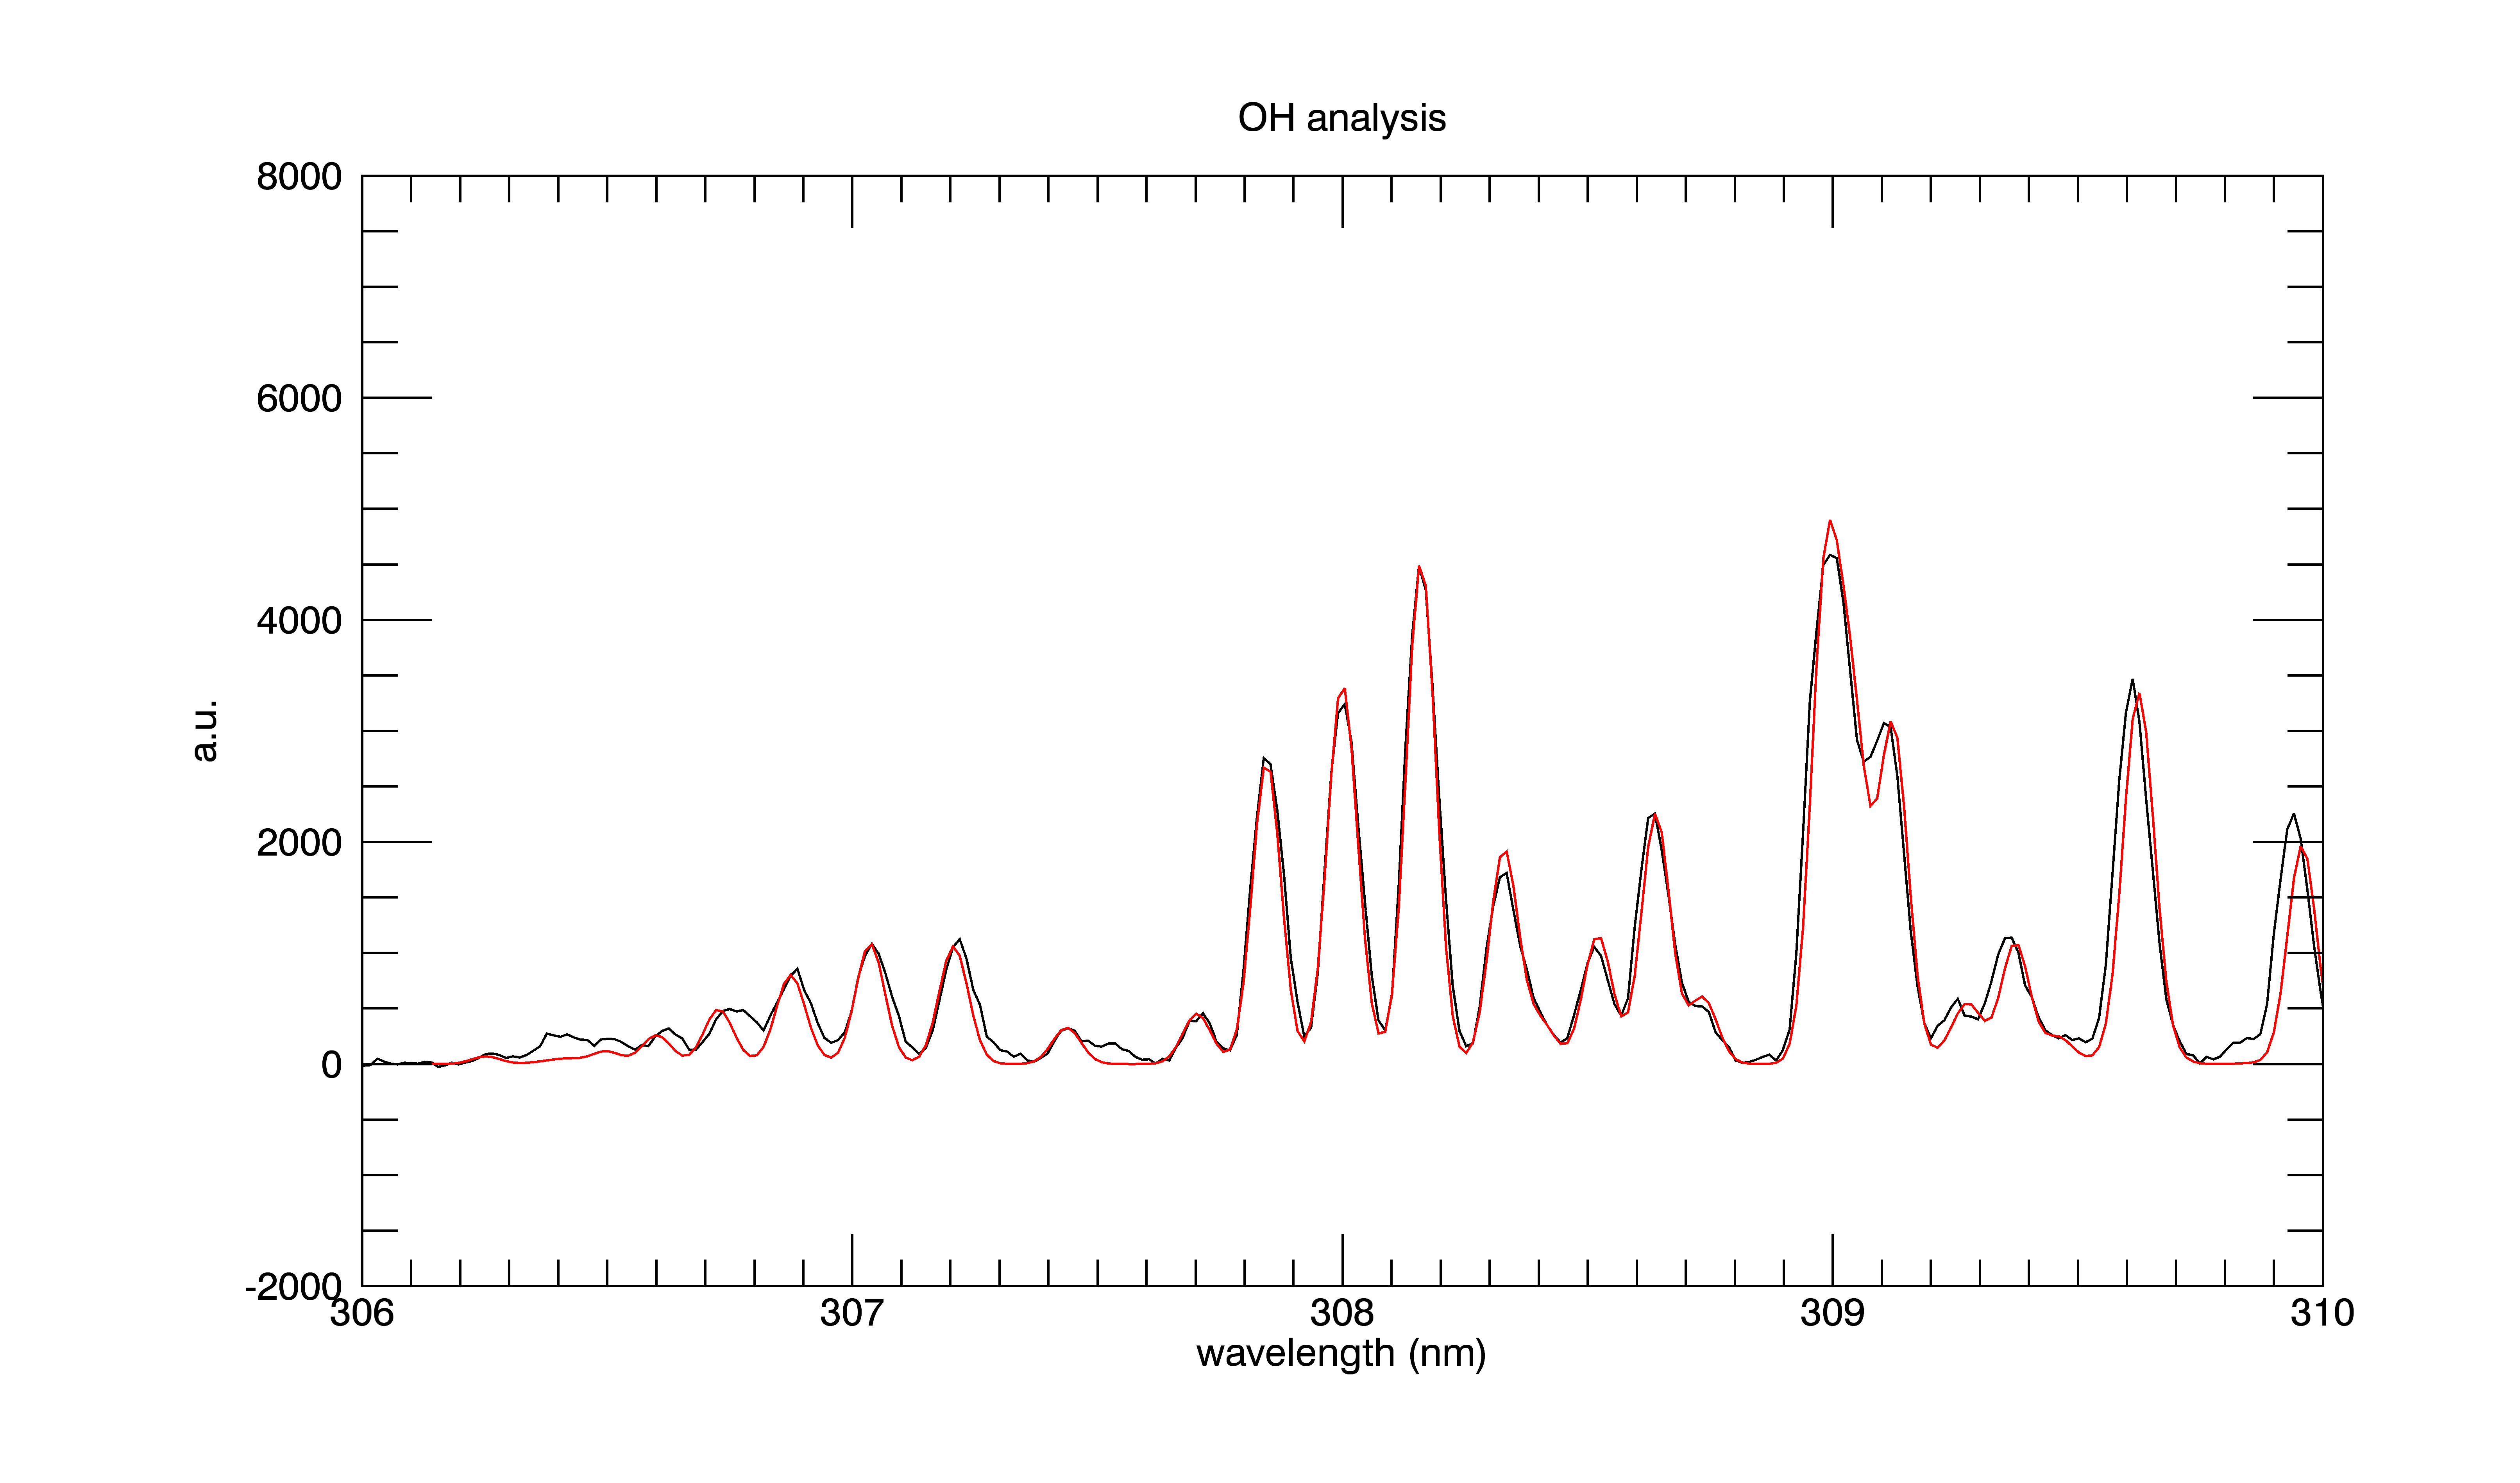
\includegraphics[width=.8\textwidth]{Immagini/OHFit_f5t16elio.png}}
 \\
 \subfloat[][\ce{N_2}]
  {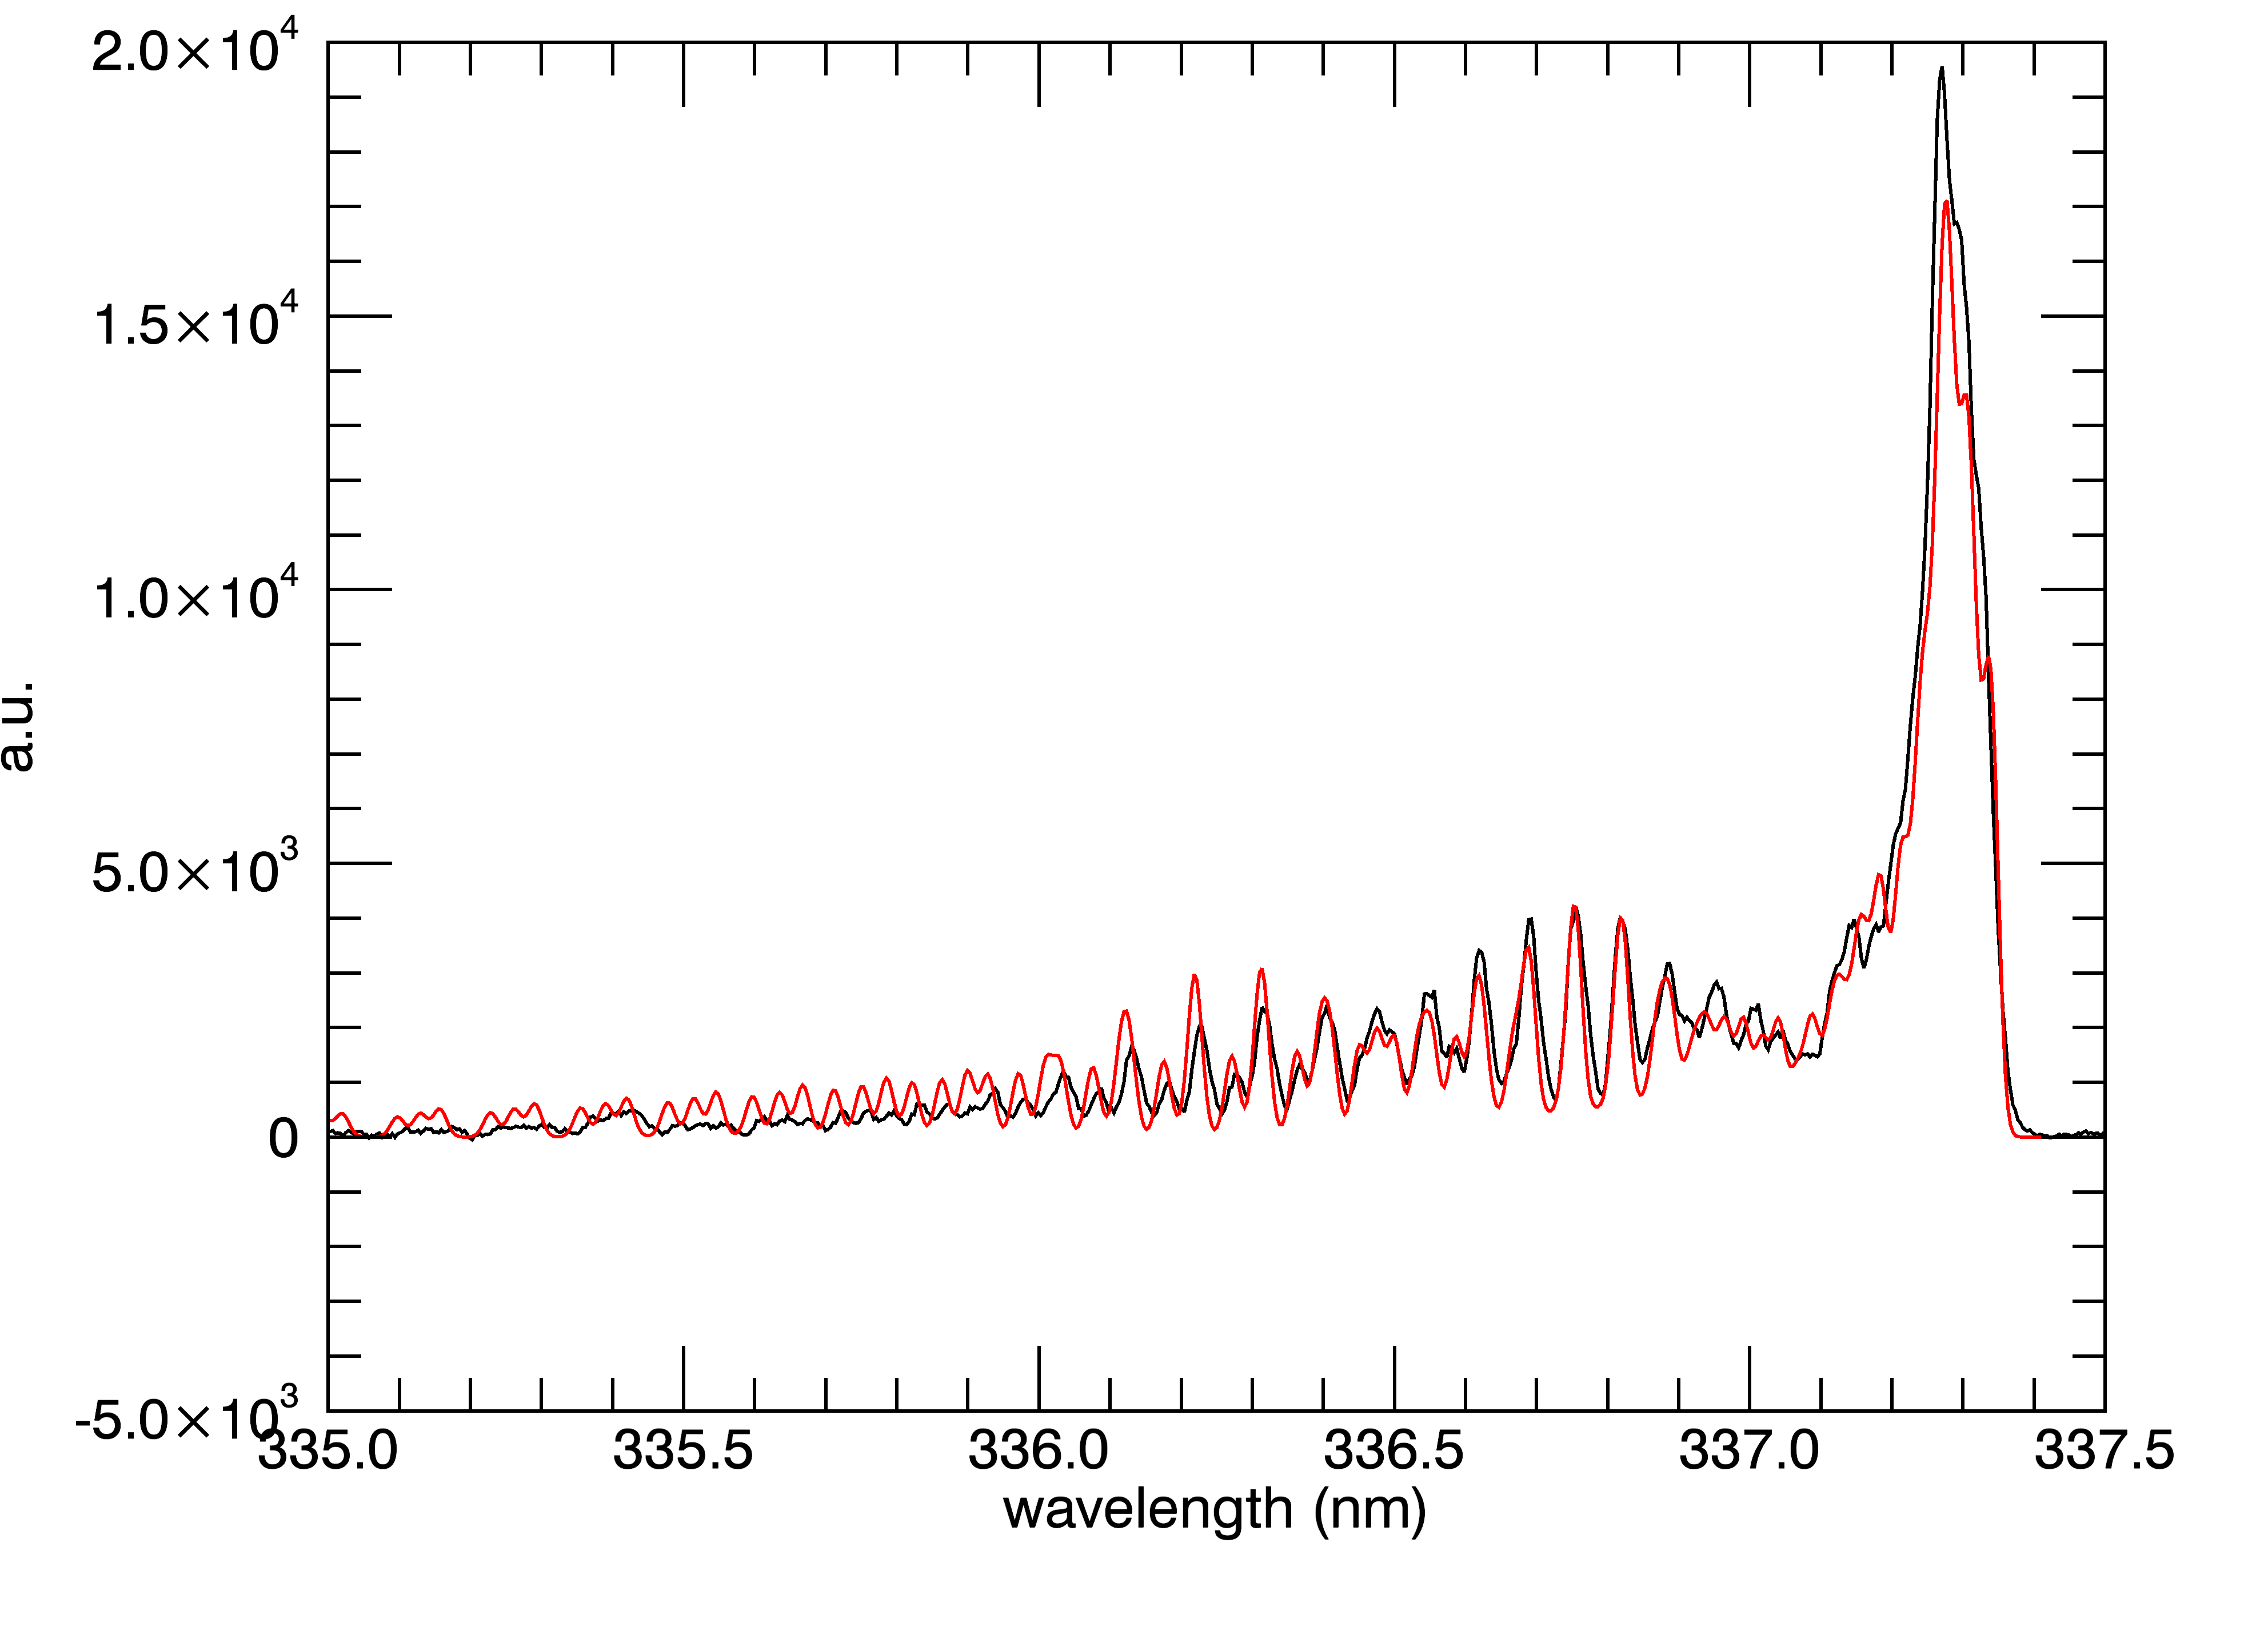
\includegraphics[width=.75\textwidth]{Immagini/N2rotFit_elio.png}}
 \caption{Fit delle emissioni con spettri simulati, misure prese con il prototipo 1, in condizioni standard, posizione 1.}
 \label{fig:fitT}
\end{figure}

\begin{table}
 \centering
 \begin{tabular}{cc}
 \toprule
            &T [\si{\kelvin}]\\
 \midrule
  \ce{OH}   &$336 \pm 30$\\
  \ce{N_2}  &$322 \pm 41$\\
 \bottomrule
 \end{tabular}
 \caption{Stima delle temperature di rotazione delle molecole.}
 \label{tab:Trot}
\end{table}
